\subsection{Dynamics results}
\label{subsec:molecular_dynamics_results}

To study the time evolution, we perform Langevin Dynamics simulation for a set of simulation parameters as described in Section~\ref{sec:simulation_details}.

The relaxation of the order parameter $S$ defined in~\eqref{eq:nematic_order_parameter} to the equilibrium value ($|S - S_{eq}|$) is shown on the Fig.~\ref{fig:op_relaxation}.

First thing to note is that notwithstanding the initial configuration, after initial rearrangement due to \textcolor{red}{Effect}, the relaxation shows the same behavior for low and moderate density for any given $k_BT$. \textcolor{red}{The random configuration is closer to equilibrium, in the sense that there are particles pointing in both directions, so I'd say that it's, like, main relaxation line, and all other initial configurations will tend to get there}. 

The results suggest power law behavior in cases of low density $\rho = 0.75$, as we can see at the left side of Fig.~\ref{fig:op_relaxation}.

For the high density, the relaxation occurs faster then for the low density. Because of this the statistical errors from Monte Carlo play greater role. To mitigate that, we simulate $1000$ samples for the long time ($t_{max} = 1000$). Using this data, we presume that system is stable after $t_{EQ} = 800$, and after performing average over samples, we time-average results after that moment. While the results \textcolor{red}{The long-time average and MC} are within the statistical error margin, \textcolor{red}{The LD gets stuck within $10^{-2} \div 10^{-2.5}$ form MC results, and do not approach any further. Also, probably this will be the case for lower densities as well, but I do not have enough long-time simulations.}

As we can see on the right side of Fig.~\ref{fig:op_relaxation}, there are distinguishable high and low $k_BT$ regimes. At the high $k_BT \geq 1.5$ the relaxation occurs \textcolor{red}{fast and with high fluctuations, so it's hard to say anything}. And there is little influence from the initial configuration. However, the low $k_BT \leq 1$ regime suggests exponential relaxation to the equilibrium results, and also it shows strong influence of initial configuration on the path and time of the relaxation. 

\begin{figure}[h]
\centering
\begin{subfigure}[t]{0.49\textwidth}
	\centering
	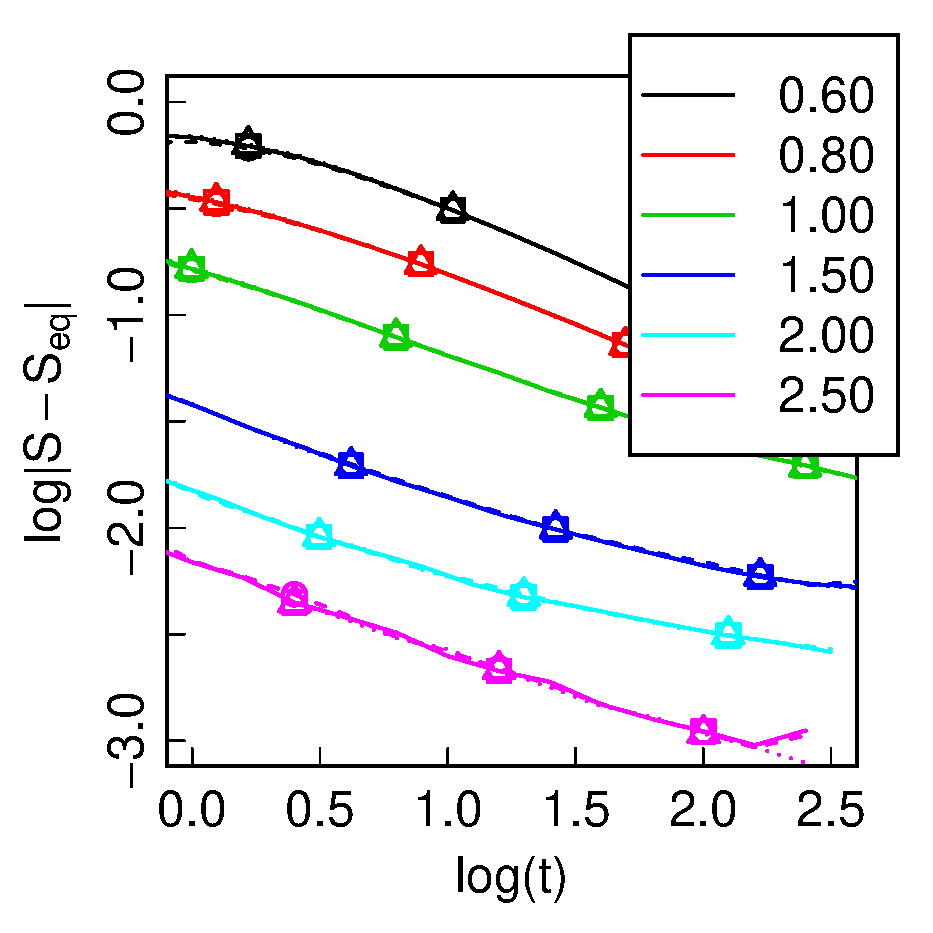
\includegraphics[width=\textwidth]{Images/relax_op_25}
%	\caption{$\rho = 0.25$}
\end{subfigure}
%\begin{subfigure}[t]{0.49\textwidth}
%	\centering
%	\includegraphics[width=\textwidth]{Images/relax_op_25_exp}
%%	\caption{$\rho = 0.25$}
%\end{subfigure}
%\begin{subfigure}[t]{0.49\textwidth}
%	\centering
%	\includegraphics[width=\textwidth]{Images/relax_op_50}
%%	\caption{$\rho = 0.50$}
%\end{subfigure}
%\begin{subfigure}[t]{0.49\textwidth}
%	\centering
%	\includegraphics[width=\textwidth]{Images/relax_op_50_exp}
%%	\caption{$\rho = 0.50$}
%\end{subfigure}
%\begin{subfigure}[t]{0.49\textwidth}
%	\centering
%	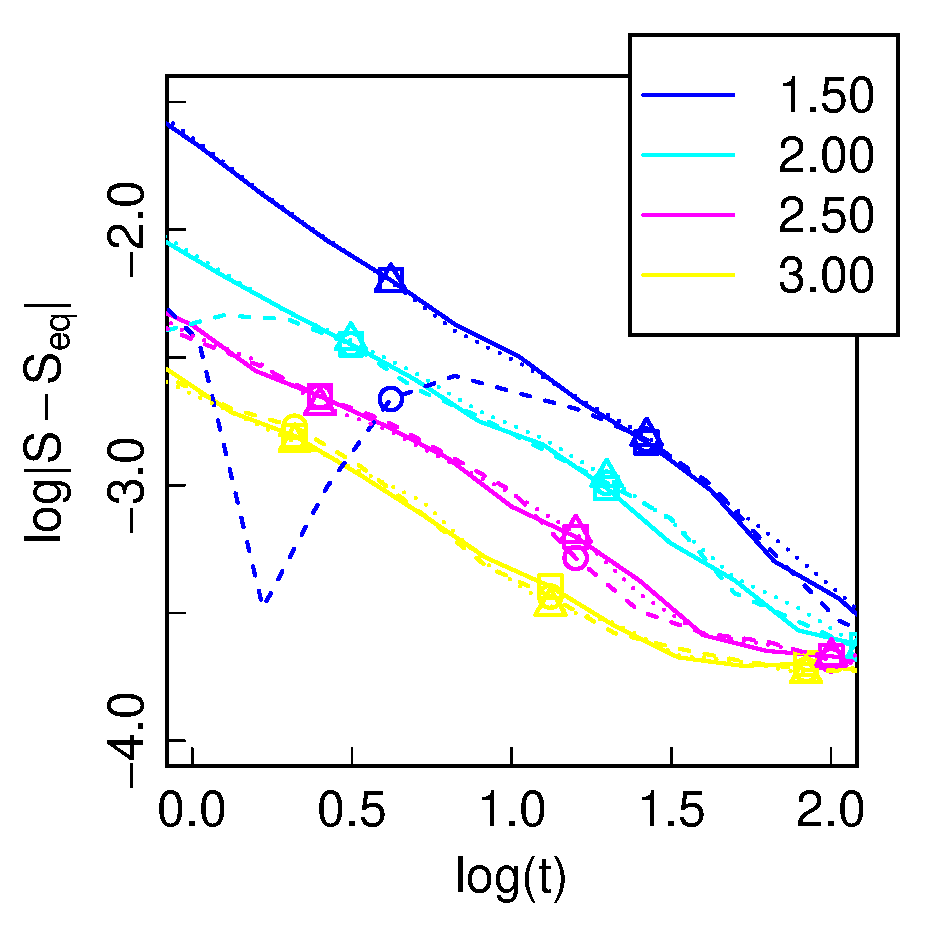
\includegraphics[width=\textwidth]{Images/relax_op_75}
%%	\caption{$\rho = 0.75$}
%\end{subfigure}
\begin{subfigure}[t]{0.49\textwidth}
	\centering
	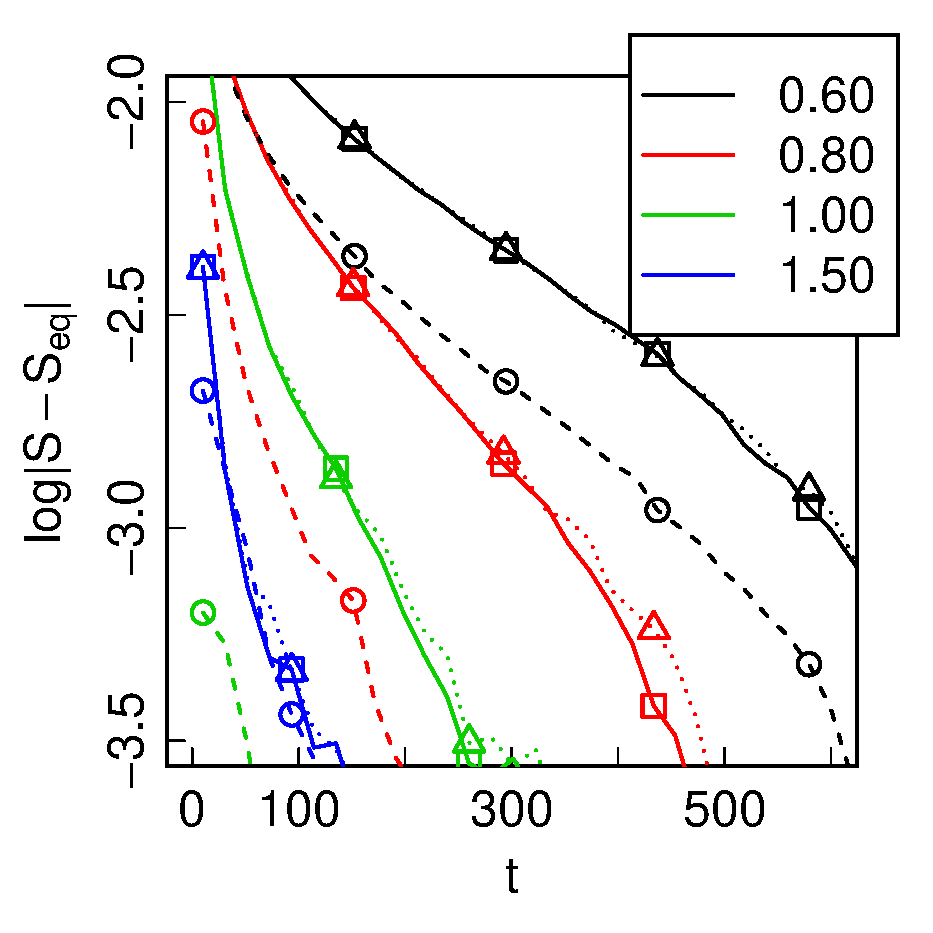
\includegraphics[width=\textwidth]{Images/relax_op_75_exp}
%	\caption{$\rho = 0.75$}
\end{subfigure}
	\captionsetup{justification=centering, width=0.9\columnwidth}
	\caption{Relaxation of order parameter to the equilibrium values for densities $\rho = 0.25, 0.75$ in the left and right respectively. The squares denote co-aligned initial configuration, and circles stand for randomly-oriented configuration. The results are obtained on $500$ samples.}
	\label{fig:op_relaxation}
\end{figure}

To gain more insight on how the system evolves, we look into particle orientations relative to its neighbors. The main results are shown at the Fig.~\ref{fig:prob_relaxation}.

First of all, we need to note that due to the symmetry of the interaction potential, the equilibrium (i.e. Monte-Carlo) results for the pairs ``LL'' -- ``RR'' and ``LR'' -- ``RL'' are the same, accounting for the statistical error.

As above, the high and low densities show different behavior. Similar to order parameter, for the low density the relaxation for any of the given orientation pairs suggests power law behavior. Also is important that there is little difference in slope of co-aligned and counter-aligned orientation pairs, as well as little influence of the $k_BT$. \textcolor{red}{add the slope values}. The respective pairs (``LL'' -- ``RR'' and ``LR'' -- ``RL'') quickly \textcolor{red}{come to the same value? and then relaxes absolutely the same way}.

For the high density the behavior is more complicated. First of all, the results suggest the exponential relaxation for prevalent (i.e. ``RR'') orientation pair, with the power strongly dependent on the $k_BT$. On the other hand, the minority orientation pair (i.e. ``LL'') relaxes differently after the initial moments. \textcolor{red}{the closer to the EQ values, the bigger the difference. It's more like power law, but unclear.}

Another observation is that co-aligned orientation pairs relaxes slower then counter-aligned. It can be attributed to their less favorable energy configuration, and therefore much lesser representation on the equilibrium.

\begin{figure}[h]
\centering
\begin{subfigure}[t]{0.49\textwidth}
	\centering
	\includegraphics[width=\textwidth]{Images/Particle_probs_25}
\end{subfigure}
\begin{subfigure}[t]{0.49\textwidth}
	\centering
	\includegraphics[width=\textwidth]{Images/Particle_probs_75}
\end{subfigure}

\begin{subfigure}[t]{0.49\textwidth}
	\centering
	\includegraphics[width=\textwidth]{Images/Particle_probs_relaxation_25}
\end{subfigure}
\begin{subfigure}[t]{0.49\textwidth}
	\centering
	\includegraphics[width=\textwidth]{Images/Particle_probs_relaxation_75}
\end{subfigure}
	\captionsetup{justification=centering, width=0.9\columnwidth}
	\caption{Relative particle orientation probabilities (top) and their relaxation to the equilibrium values (bottom), for low ($\rho = 0.25$) and high ($\rho = 0.75$) density at the left and right respectively. Lines show the equilibrium results, however, the pairs ``LL'' -- ``RR'' and ``LR'' -- ``RL'' values are indistinguishable at this scale. The simulations start from co-aligned initial configuration.}
	\label{fig:prob_relaxation}
\end{figure}
	
The average autocorrelation of the particles orientation as the function of time is shown at the Fig.~\ref{fig:autocorrelation}. The results clearly shows the exponential tail for any given $k_BT$ and density. However for short time scale the behaviour isn't exponential. The exponential tail gives us the following relation: $C(t) \sim \exp[t/t^*]$, where $t^*$ is the autocorrelation time. If we look how it depends on density and $k_BT$, we obtain the results shown at the Fig.~\ref{fig:autocorrelation_time}. We want to note here that the correlation time is longer for the co-aligned then it is for the random initial configuration, however, with increase in density the ratio between the two decreases. \textcolor{red}{Need to check the 0.5 results, probably naming error}.

\begin{figure}[p]
\centering
	\begin{subfigure}[t]{0.49\textwidth}
		\centering
		\includegraphics[width=\textwidth]{Images/corr_time_relaxation_25.png}
		\caption{$\rho = 0.25$}
	\end{subfigure}
	\begin{subfigure}[t]{0.49\textwidth}
		\centering
		\includegraphics[width=\textwidth]{Images/corr_time_relaxation_75.png}
		\caption{$\rho = 0.75$}
	\end{subfigure}
	\captionsetup{justification=centering, width=0.9\columnwidth}
	\caption{Autocorrelation of particles orientation as function of time for LD simulations. The points are obtained as described in sec.~\ref{sec:simulation_details}. The squares correspond to random, and the circles corresponds to co-aligned initial configuration. Lines are the linear approximation to the data. \textcolor{red}{I selected regions by hand, which looks the most linear, how can I say that?}. Inset shows the results over bigger time frame.}
	\label{fig:autocorrelation}
\end{figure}



\begin{figure}[h]
\centering
	\includegraphics[width=0.49\textwidth]{Images/time_corrs_dif_kbt.png}
	
	\captionsetup{justification=centering, width=0.9\columnwidth}
	\caption{Correlation time for Langevin Dynamics simulations as function of $k_BT$ and density. The squares correspond to random, and the circles corresponds to co-aligned initial configuration.} 
	\label{fig:autocorrelation_time}
\end{figure}



